\documentclass[11pt]{beamer}

\usetheme{Singapore}
\usepackage[utf8]{inputenc}
\usepackage{amsmath}
\usepackage{amsfonts}
\usepackage{amssymb}
\usepackage{graphicx}
\usepackage{hyperref}

% Setup the bibliography
\usepackage[style=authortitle,backend=bibtex]{biblatex}
\addbibresource{bibliography.bib}
\setbeamertemplate{bibliography item}[text]
\setbeamerfont{footnote}{size=\tiny}

\author{Steve Pederson}
\title{Lecture 1: Introduction to the Transcriptome}
\subtitle{BIOINF3005/7160: Transcriptomics Applications}
%\setbeamercovered{transparent} 
\setbeamertemplate{navigation symbols}{} 
\logo{
	\includegraphics[scale=0.3]{figures/UoA_logo_col_vert.png} 
} 
\institute{University of Adelaide} 
\date{March 2nd, 2020} 
\subject{BIOINF3005/7160: Transcriptomics Applications} 


\begin{document}

\begin{frame}
\titlepage
\end{frame}

\begin{frame}
\tableofcontents
\end{frame}

\section{Introduction}

\subsection{Important Information From The University}

\begin{frame}{Welcome to the University of Adelaide}

	\begin{itemize}
		\item The start of any academic year is an exciting time - but it can also be challenging for our students, for many reasons
		\item For some of our students, this year is especially challenging
		\item That’s because many of our students who wanted to be here to study can’t be here - because of COVID-19 and the travel restrictions to Australia
		\item This is not a situation that those students - or any of us in this room today - have any direct control over
		\item We may have some students watching this very lecture from overseas
	\end{itemize}
	
\end{frame}

\begin{frame}{Welcome to the University of Adelaide}

	\begin{itemize}
		\item Before the lecture begins, there are some points worth making so that everyone understands what the current situation is here at the University of Adelaide
		\item We have a diverse, inclusive, and welcoming community at our University, which is something we’re very proud of
		\item In times of difficulty, that community is more important than ever.
		\item This is a time when our community comes together as a whole so we can care for and support each other together
		\item It’s particularly important for those who may be going through a more difficult time than otherwise. 
		\item We must be respectful of other people - and that includes the many students who couldn’t join us in the room today
	\end{itemize}

\end{frame}

\begin{frame}{COVID-19}

	\begin{itemize}
		\item The impact of COVID-19 is being felt right around the world. 
		\item The University’s own response to COVID-19 is being shaped by the latest advice from the Government and from health authorities. 
		\item So far, there have only been a small number of COVID-19 cases in Australia ... only three in South Australia  ... and none at the University.	
		\item There is no evidence of transmission within the general community in Australia.
		\item Health authorities are advising we take the same basic precautions we would when it’s cold or flu season – wash your hands, cover your mouth, dispose of tissues.
		\item This is good advice for any time you have a cough or a cold.	
 
	\end{itemize}

\end{frame}

\begin{frame}{COVID-19}

	\begin{itemize}
		\item There are resources available for students who need someone to talk to:
		
		\begin{itemize}
			\item Student Life, if you need some extra assistance or support
			\item Our Safer Campus Community website has a lot of resources to help us address harassment, including ways to report and get help
			\item Adelaide UniCare is our on-campus medical service, and you can make appointments online.
		\end{itemize}
		
		\item The University also has an online FAQ page about COVID-19 that’s being constantly updated - there’s a banner on our main webpage that links to the FAQ.
		\item The University has made it very clear that the safety and well-being of staff and students is paramount, and we will communicate with you clearly if anything changes.
		\item Welcome again, and good luck with your studies.
	\end{itemize}

\end{frame}


\subsection{Course Details}

\linespread{1.2}

\begin{frame}{Course Timetable}

	\begin{itemize}
		\item Lectures:
		\begin{itemize}
			\item Monday 9:10am - 10:00am, Room B18, Ingkarni Wardli
\end{itemize}		 
		\item Practicals:
		\begin{itemize}
			\item Wednesday 9:10am - 11:00am, Room 111, Johnson Building
			\item Friday 9:10am - 11:00am, Room 111, Johnson Building
		\end{itemize}
	\end{itemize}

\end{frame}

\begin{frame}{Course Outline}

	\begin{itemize}
		\item Discussion of underlying biology
		\item Experimental approaches utilised in transcriptomic analysis
		\item Statistical and computational approaches utilised in transcriptomic analysis
		\item Praticals will be entirely computational
		\begin{itemize}
			\item Focussed on working in \texttt{R} with some \texttt{bash}
		\end{itemize}
	\end{itemize}

\end{frame}

\begin{frame}{Assessment}

	\begin{itemize}
		\item Continuous Assessment (\textit{i.e. no exam})
		\item 6 assignments (+ Major Project for Bioinf7160)
		\item Assessment is strongly focussed on practical material
		\item Attendance at practicals is not compulsory, but is \textbf{strongly advised}
	\end{itemize}

\end{frame}

\begin{frame}{Results from 2019 (BIOTECH7005)}

	\begin{center}
	\includegraphics[scale=0.5]{figures/biotech7005_2019pca.pdf} 	
	\end{center}


\end{frame}

\section{Why Study the Transcriptome?}

\linespread{1.05}

\subsection{What is the Transcriptome}

\begin{frame}{The Transcriptome}

	\begin{block}{Definition}
	The transcriptome can be defined as the complete set of transcripts in a cell, or a population of cells, for a specific developmental stage or physiological condition\footfullcite{pmid19015660}
	\end{block}
	

\end{frame}

\begin{frame}{The Transcriptome}

	This can be summarised as the \textit{RNA content of a cell}.\\[3mm]
	
	\begin{itemize}
		\item Can include messenger RNA (\textit{mRNA}), non-coding RNA (\textit{ncRNA}), small RNA (\textit{miRNA, piRNA etc.})
		\item Can also include transfer RNA (\textit{tRNA}) and ribosomal RNA (\textit{rRNA}), but this is less common
	\end{itemize}
	
	\vspace{3mm}
	
	We are always dealing with a \textbf{snapshot of a dynamic process}

\end{frame}

\begin{frame}{Why Study The Transcriptome?}

	\begin{itemize}
		\item \textit{mRNA} is the intermediary step between the genome (DNA) and proteins
		\item small RNA and \textit{ncRNA} play significant roles in gene regulation
		\item Make inference about the \textbf{biological processes driving our observations}
		\begin{itemize}
			\item Targets for curing disease
			\item Biomarkers for tumour detection
			\item Understanding drought/salinity tolerance
		\end{itemize}

	\end{itemize}
	
\end{frame}

\subsection{The Central Dogma}

\begin{frame}{The Central Dogma of Molecular Biology}

	A common (but simplistic) version of the Central Dogma:
	
	\vspace{3mm}	
	
	\begin{center}
	\includegraphics[scale=1]{figures/Watson_Central_Dogma.jpg} 	
	\end{center}
	
	\vspace{3mm}	
	
	\begin{block}{}
	DNA makes RNA makes Protein.
	(Figure taken from \textit{The Molecular Biology of the Gene}\footfullcite{watson1965}, p298)
	\end{block}
	
	
\end{frame}

\begin{frame}{The Central Dogma of Molecular Biology}

	According to Crick\footfullcite{crick1956} 

	\begin{center}
	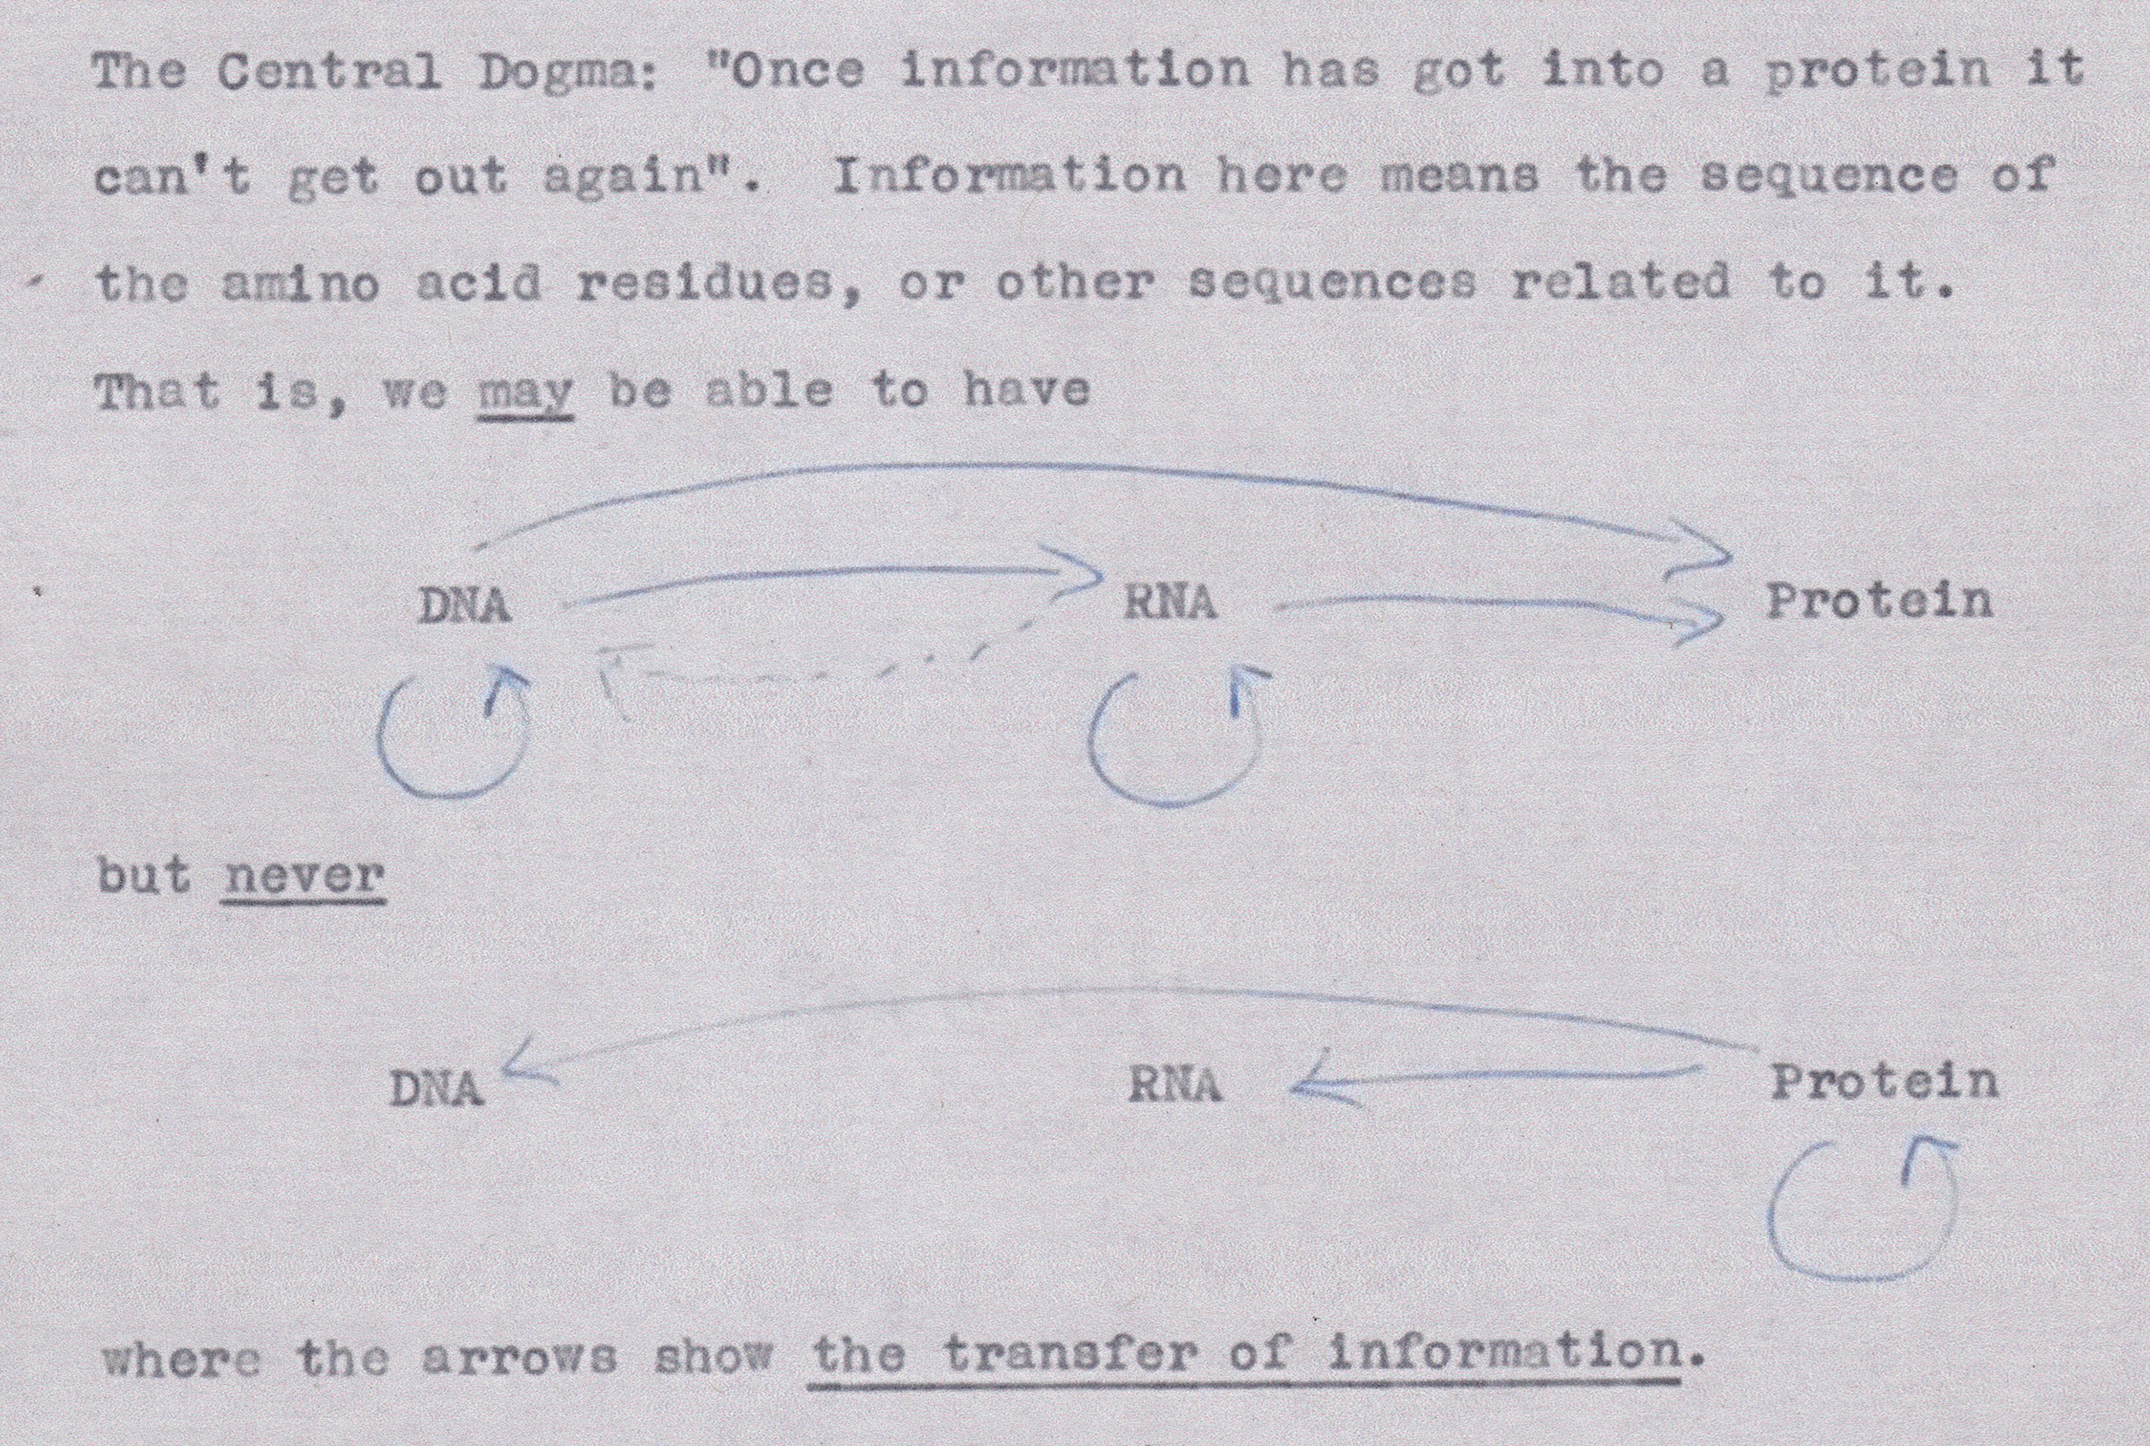
\includegraphics[scale=0.45]{figures/crick_dogma_note.png}
	\end{center}
	

\end{frame}

\section{Key Definitions}

\subsection{What is a Gene?}

\begin{frame}{What is a Gene?}

	\begin{block}{Definition}
		The gene is the basic physical unit of inheritance. 
		Genes are passed from parents to offspring and contain the information needed to specify traits. 
		Genes are arranged, one after another, on structures called chromosomes. 
		A chromosome contains a single, long DNA molecule, only a portion of which corresponds to a single gene. 
		Humans have approximately 20,000 genes arranged on their chromosomes.\footnote{https://www.genome.gov/genetics-glossary/Gene}
	\end{block}
	
\end{frame}


\begin{frame}{What is a Gene?}

	\begin{itemize}
		\item Classically, a \textit{gene} is a genomic locus that is \textbf{transcribed from DNA into RNA}\footnote{NB: This definition does not include chimeric transcripts from more than one DNA locus}
		\item Some genes are protein coding, others are not
		\item A gene may have numerous \textit{transcripts}, or \textit{isoforms}
		
		\begin{itemize}
			\item Some transcripts of a gene may be protein coding
			\item Some transcripts from \textit{the same gene} may not be protein coding		
		\end{itemize}
		
	\item Genes can range in size from dozens to millions of nucleotides

	\end{itemize}
	
\end{frame}

\begin{frame}{What is a Gene?}

	Here is an example region on the human X chromosome\footnote{\href{https://genome.ucsc.edu/cgi-bin/hgTracks?db=hg38\&lastVirtModeType=default\&lastVirtModeExtraState=\&virtModeType=default\&virtMode=0\&nonVirtPosition=\&position=chrX\%3A49186416\%2D49289908\&hgsid=804874837\_yhlSH5Dok8PNRGEWxk6lc7auhaeK}{UCSC Genome Browser}}
	\vspace{5mm}

	\begin{center}
	\includegraphics[scale=0.11]{figures/ucscExample.png} 	
	\end{center}

\end{frame}

\subsection{What is Transcription?}

\begin{frame}{What is Transcription?}

	\begin{block}{Transcription}
		Transcription is the process of making an RNA copy of a gene sequence\footnote{https://www.genome.gov/genetics-glossary/Transcription?id=197}
	\end{block}

	\begin{center}
	\includegraphics[scale=0.14]{figures/transcription.jpg} 
	\end{center}

\end{frame}

\begin{frame}{The Steps of Transcription}

	\begin{enumerate}
		\item RNA polymerase, together with one or more transcription factors, \textbf{binds to the promoter}
		\item RNA polymerase creates a transcription bubble, which \textbf{separates the two strands of the DNA helix}, breaking the hydrogen bonds between complementary DNA nucleotides.
		\item RNA polymerase \textbf{adds RNA nucleotides} complementary to the nucleotides of one DNA strand.
		\item RNA sugar-phosphate backbone forms to create \textbf{single-stranded RNA}.
		\item Hydrogen bonds of the RNA–DNA complex break, \textbf{freeing the newly synthesized RNA strand}.\\
	\end{enumerate}

\end{frame}

\begin{frame}{The Steps of Transcription}

If the cell has a nucleus (i.e. a \textit{eukaryotic cell}): \\

	\begin{enumerate}
	\setcounter{enumi}{5}

		\item The RNA may be further processed. This may include \textbf{polyadenylation}, \textbf{capping}, and \textbf{splicing}.
		\item The RNA may remain in the nucleus or \textbf{exit to the cytoplasm} through the nuclear pore complex.
	\end{enumerate}
	
\textbf{Before transcription even starts}, the relevant section of DNA must be unpacked from any histones

\end{frame}

\subsection{What is a Promoter?}

\begin{frame}{What is a Promoter?}

	\begin{block}{Definition}
	A promoter is a region of DNA that leads to initiation of transcription of a particular gene. 
	Promoters are located near the transcription start sites of genes, upstream on the DNA (towards the 5' region of the sense strand). \footnote{https://en.wikipedia.org/wiki/Promoter\_(genetics)}
	\end{block}

\end{frame}

\begin{frame}{Key Elements of a Eukaryotic Promoter}

The \textbf{core promoter} is the minimal portion of the promoter required to properly initiate transcription.

	\begin{itemize}
		\item Includes the transcription start site (TSS) and elements directly upstream
		\item A binding site for RNA polymerase
		\item General transcription factor binding sites, e.g. TATA box, B recognition element.
		\item Many other elements/motifs may be present. 
			There is no such thing as a set of "universal elements" found in every core promoter.
	\end{itemize}

\end{frame}

\begin{frame}{Key Elements of a Eukaryotic Promoter}

The \textbf{Proximal promoter} is the proximal sequence upstream of the gene that tends to contain primary regulatory elements

	\begin{itemize}
		\item Approximately 250 base pairs upstream of the start site
		\item Specific transcription factor binding sites
	\end{itemize}

The \textbf{Distal promoter} is the distal sequence upstream of the gene often with a weaker influence than the proximal promoter

	\begin{itemize}
		\item Additional (weaker) regulatory elements, 
		\item Anything further upstream (but not an enhancer or other regulatory region whose influence is positional/orientation independent)
		\item Specific transcription factor binding sites
	\end{itemize}

\end{frame}



\begin{frame}{}

	\begin{itemize}
		\item 
	\end{itemize}

\end{frame}

\end{document}
